\documentclass[11pt,a4paper,oneside]{book}
%-- coding: UTF-8 --
\usepackage[UTF8]{ctex}
\usepackage{fontspec}
\defaultfontfeatures{Mapping=tex-text}
\usepackage{xunicode}
\usepackage{xltxtra}
\usepackage{amsmath}
\usepackage{amsfonts}
\usepackage{amssymb}
\usepackage{graphicx}
\usepackage{amsthm}
\usepackage{array}
\usepackage{float}   %{H}
\usepackage{booktabs}  %\toprule[1.5pt]
\setcounter{secnumdepth}{4}
\usepackage{indentfirst} %首行缩进
\usepackage{tcolorbox} %彩色框框
\usepackage{graphicx}  %图片并排
\usepackage{subfigure} %图片并排
\usepackage{graphicx} %插入jpg
\setcounter{secnumdepth}{4}		%增加编号深度
\setcounter{tocdepth}{4}		%增加目录深度
\usepackage{hyperref}     %生成pdf书签
\hypersetup{hidelinks,
	colorlinks=true,
	allcolors=black,
	pdfstartview=Fit,
	breaklinks=true
}       %去掉目录的红色框框
%===================%插入代码需要的控制
\usepackage{listings}
\usepackage{xcolor}
\setmonofont{Consolas}%字体
\lstset{
	numbers=left, 
	numberstyle= \tiny, 
	keywordstyle= \color{ blue!70},
	commentstyle= \color{red!50!green!50!blue!50}, 
	frame=shadowbox, % 阴影效果
	rulesepcolor= \color{ red!20!green!20!blue!20} ,
	escapeinside=``,% 英文分号中可写入中文
	basicstyle=\ttfamily 
} 
%===================%
\usepackage[left=2cm,right=2cm,top=2cm,bottom=2cm]{geometry}
\newtheorem{theorem}{定理}
\newtheorem{definition}{定义}
\pagestyle{plain}%设置页码
\title{\huge NOTE on TimeSeries \& R}
\author{zy}
\date{\today}

\begin{document}
	\maketitle
	\tableofcontents  %目录

\chapter{时间序列概念}
\section{时间序列的分解}
\subsection{例:北京地区洪涝灾害数据}

\begin{lstlisting}[language=r]
> flood.data <- matrix(c(
+   1949 , 1 , 331.12 , 243.96 , 
+   1950 , 2 , 380.44 , 293.90 , 
+   1951 , 3 , 59.63 , 59.63,
+   1952 , 4 , 37.89 , 18.09,
+   1953 , 5 , 103.66 ,72.92,
+   1954 , 6 , 316.67 , 244.57,
+   1955 , 7 , 208.72 , 155.77,
+   1956 , 8 , 288.79 , 255.22,
+   1957 , 9 , 25.00 , 0.50,
+   1958 , 10 , 84.72 , 48.59,
+   1959 , 11 , 260.89 ,202.96,
+   1960, 12 , 27.18 ,15.02,
+   1961, 13 , 20.74 ,17.09,
+   1962 , 14 , 52.99 ,14.66,
+   1963 , 15 , 99.25 , 45.61,
+   1964 , 16 , 55.36 ,41.90),
+   byrow=T, ncol=4,
+   dimnames=list(1949:1964, c("year", "t", "area1", "area2")))
\end{lstlisting}
\begin{tcolorbox}[colback=pink!10!white,colframe=pink!100!black]
\textbf{matrix(data, nrow, ncol, byrow, dimnames)}
\begin{itemize}
	\item 数据是成为矩阵的数据元素的输入向量。
	\item nrow是要创建的行数。ncol是要创建的列数。
	\item byrow是一个逻辑线索。 如果为TRUE,则输入向量元素按行排列。
	\item dimname是分配给行和列的名称。
\end{itemize}
\end{tcolorbox}

\begin{lstlisting}[language=r]
> flood.area1 <- ts(flood.data[,"area1"],
+                   frequency=1,
+                   start=1949)
> flood.area2 <- ts(flood.data[,"area2"],
+                   frequency=1,
+                   start=1949)
\end{lstlisting}
\begin{tcolorbox}[colback=pink!10!white,colframe=pink!100!black]
\textbf{timeseries.object.name <-  ts(data, start, end, frequency)}
	\begin{itemize}
		\item data是包含在时间序列中使用的值的向量/矩阵。除了参数data,所有其他参数是可选的。
		\item start以时间序列指定第一次观察的开始时间。
		\item end指定时间序列中最后一次观测的结束时间。
		\item frequency指定每单位时间的观测数。
	\end{itemize}
\end{tcolorbox}

\begin{lstlisting}[language=r]
> fig.flood <- function(){
	+   opar <- par(mar=c(3,3,2,1), mgp=c(1.5,0.5,0))
	+   on.exit(par(opar))
	+   plot(flood.area1, lty=1, type="b",
	+        main=' 洪水灾害数据',
	+        xlab=' 年', ylab=' 面积(万亩)')
	+   lines(flood.area2, lty=2, type="b")
	+   legend("topright", lty=c(1,2), legend=c('受灾面积', '成灾面积'))
	+ }
> fig.flood()
\end{lstlisting}
\begin{figure}[H]
	\centering
	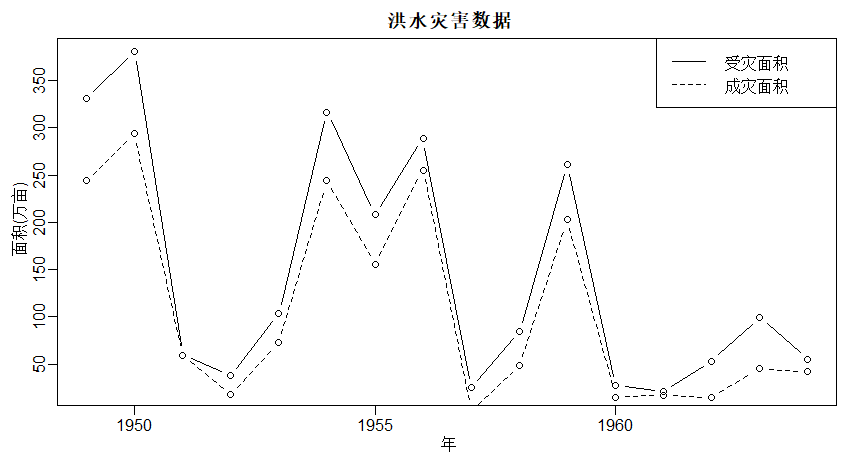
\includegraphics[width=0.7\textwidth]{1.png}
\end{figure}
在R语言做图中,可以简单的通过配置参数达到想要的效果,但是参数有很多,有必要进行分类,避免滥用或浪费。比如有一些参数如颜色大小是可以通用的,被分到了par里面,作为公共参数集合;还有一些如坐标轴就只能有类似plot这样的函数保有,给别人人家也用不到那些啊。如果plot的坐标轴要用颜色相关的属性,那么就可以直接去par中取来用就是了。如果title想用字体这个属性,也可以去par中取。所以par理所当然的可以被称为公共参数列表了。

\textbf{opar <- par(no.readonly=TRUE)}这个语句。这个语句保存了之前的默认参数.

\begin{tcolorbox}[colback=pink!10!white,colframe=pink!100!black]
\textbf{opar <- par(mar=c(3,3,2,1), mgp=c(1.5,0.5,0))}

\textbf{mar}\\
A numerical vector of the form c(bottom, left, top, right) which gives the number of lines of margin to be specified on the four sides of the plot. The default is c(5, 4, 4, 2) + 0.1.
当出现轴标题与轴标注发生重叠时,可以手动设置mar来解决.

使用\textbf{mgp}=c(5,1,0)把轴标题设置距离图形区域5,轴标签设置为1,轴本身为0,单位为行高【默认mgp=c(3, 1, 0)】
\end{tcolorbox}

\begin{tcolorbox}[colback=pink!10!white,colframe=pink!100!black]
\textbf{	on.exit(expr = NULL, add = FALSE, after = TRUE)}
	\begin{itemize}
		\item expr: an expression to be executed.
		\item add: if TRUE, add expr to be executed after any previously set expressions (or before if after is FALSE); otherwise (the default) expr will overwrite any previously set expressions.
		\item after: if add is TRUE and after is FALSE, then expr will be added on top of the expressions that were already registered. The resulting last in first out order is useful for freeing or closing resources in reverse order.
	\end{itemize}
\end{tcolorbox}

\begin{tcolorbox}[colback=pink!10!white,colframe=pink!100!black]
	\textbf{plot(v,type,col,xlab,ylab)}
	\begin{itemize}
		\item v是包含數值的向量。
		\item 類型採用值“ p”僅替換點,“ l”僅替換線和“ o”替換點和線。
		\item xlab是x軸的標籤。ylab是y軸的標籤。
		\item main是圖表的標題。
		\item col用作給點和線的顏色。
	\end{itemize}

通過使用\textbf{lines()}函數,可以在同一個圖表上繪製多條線。
\end{tcolorbox}
\textbf{legend(x, y = NULL, legend, fill = NULL, col = par("col"),
border = "black", lty, lwd, pch,
angle = 45, density = NULL, bty = "o", bg = par("bg"),
box.lwd = par("lwd"), box.lty = par("lty"), box.col = par("fg"))}\\


Arguments | 参数

x, y:用于定位图例,也可用单键词"bottomright", "bottom", "bottomleft", "left", "topleft", "top", "topright", "right" and "center"

legend:字符或表达式向量

fill:用特定的颜色进行填充

col:图例中出现的点或线的颜色

border:当fill = 参数存在的情况下,填充色的边框

lty, lwd:图例中线的类型与宽度

pch:点的类型

angle:阴影的角度

density:阴影线的密度

bty:图例框是否画出,o为画出,默认为n不画出

bg:bty != "n"时,图例的背景色

box.lty, box.lwd, box.col

bty = "o"时,图例框的类型,box.lty决定是否为虚线,box.lwd决定粗线,box.col :决定颜色\\


Example | 例子

> legend("topleft", inset=.05, title="Drug Type", c("A","B"),
+        lty=c(1, 2), pch=c(15, 17), col=c("red", "blue"))

\subsection{例:居民用煤消耗季度值}
\begin{lstlisting}[language=r]
> coal.consumption <-
+     ts(c(
+         6878.4 , 5343.7 , 4847.9 , 6421.9 ,
+         6815.4 , 5532.6 , 4745.6 , 6406.2 ,
+         6634.4 , 5658.5 , 4674.8 , 6445.5 ,
+         7130.2 , 5532.6 , 4989.6 , 6642.3 ,
+         7413.5 , 5863.1 , 4997.4 , 6776.1 ,
+         7476.5 , 5965.5 , 5202.1 , 6894.1 ),frequency=4, start=c(1991,1))
\end{lstlisting}

\begin{lstlisting}[language=r]
> demo.coal.data <- function(){
	+     opar <- par(mar=c(3,3,3,1), mgp=c(1.5,0.5,0))
	+     on.exit(par(opar))
	+     plot(coal.consumption, lty=1, type='b',
	+          main=' 居民季度用煤消耗量',
	+          xlab=' 年', ylab=' 消耗量(吨)')
	+     abline(v=1991:1996, lty=3)
	+ }
> demo.coal.data()
\end{lstlisting}
\begin{figure}[H]
	\centering
	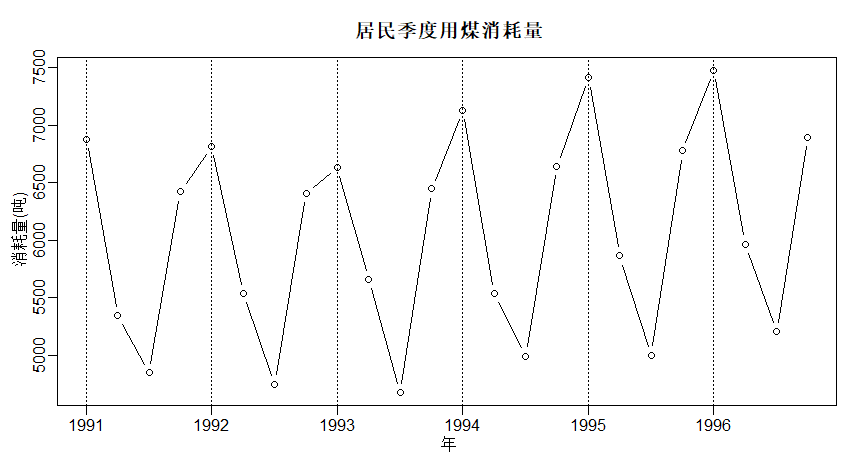
\includegraphics[width=0.7\textwidth]{2.png}
\end{figure}
\subsubsection{用每年的平均值作为趋势项估计, 季度平均作为季节项}
这样的趋势是阶梯函数,每年的4 个季度的趋势相等。去趋势后同季度平均作
为季节项。

\begin{lstlisting}[language=r]
> y <- coal.consumption
> ymore <- ts(c(y, rep(NA,4)), start=start(y), frequency=4)
> ymat <- matrix(c(y), byrow=TRUE, nrow=6, ncol=4)
> cols <- rainbow(20)
> ic <- 1


> ## 用同季度的值平均得到四个季节项--季节项得求取函数设计
> get.season <- function(yd){ # input: Detrended series
	+     ymat <- matrix(c(yd), byrow=TRUE, ncol=4)
	+     ## 季节项求取
	+     seas0 <- apply(ymat, 2, mean, na.rm=TRUE)
	+     seas0
	+ }

> ## 画去除趋势后的序列、季节项和随机项
> plot.season <- function(yd, seas0){ # input Detrended series用已除趋势项的序列
	+     ## 季节项
	+     seas <- rep(seas0, 6)
	+     seas <- ts(seas, start=c(1991,1), frequency=4)
	+     ## 随机项
	+     r <- c(yd) - seas
	+     r <- ts(r, frequency=4, start=c(1991,1))
	+     plot(yd, type='b', lwd=2,
	+          main="Detrended Series(black), Seasonal(red) and Random(cyan)",
	+          xlim=c(1991,1998), ylab="")
	+     abline(v=1991:1996, col="gray")
	+     abline(h=0, col="gray")
	+     lines(seas, type="l", col="red")
	+     lines(r, type="l", col="cyan")
	+ }
\end{lstlisting}

\begin{tcolorbox}[colback=pink!10!white,colframe=pink!100!black]
	\textbf{rep(x, time = , length = , each = ,)}
	\begin{itemize}
		\item x:代表的是你要进行复制的对象,可以是一个向量或者是一个因子。
		\item times:代表的是复制的次数,只能为正数。负数以及NA值都会为错误值。复制是指的是对整个向量进行复制。
		\item each:代表的是对向量中的每个元素进行复制的次数。
		\item length.out:代表的是最终输出向量的长度。 
	\end{itemize}
\end{tcolorbox}
\begin{tcolorbox}[colback=pink!10!white,colframe=pink!100!black]
	\textbf{rainbow(n, s = 1, v = 1, start = 0, end = max(1, n - 1)/n, alpha = 1)}

例如,基于彩虹色渐变获取10个颜色,依次由red、yellow、green、cyan、green、blue 、magenta等顺序细化而成:rainbow(10)
\end{tcolorbox}
\begin{tcolorbox}[colback=pink!10!white,colframe=pink!100!black]
	\textbf{apply(array, margin, FUN, ...)}
	\begin{itemize}
		\item 在array上,沿margin方向,依次调用FUN。返回值为vector。
		\item margin表示数组引用的第几维下标(即array[index1, index2, ...]中的第几个index),1对应为1表示行,2表示列,c(1,2)表示行列。
	\end{itemize}
\end{tcolorbox}

下图为原始序列、趋势、拟合(包括趋势与季节项):
\begin{lstlisting}[language=r]
> tr0 <- apply(ymat, 1, mean, na.rm=TRUE)          #趋势项
> tr <- rep(tr0, each=4)
> tr <- ts(tr, frequency=4, start=c(1991,1))

> y.detrended <- y - tr                            #去除趋势
> seas0 <- get.season(y.detrended)                 #求季节项

> tr.more <- ts(c(tr, rep(tr[length(tr)],4)),
+               start=start(y), frequency=4)
> seas.more <- ts(rep(seas0, 7),
+                 start=start(y), frequency=4)
> y.pred <- tr.more + seas.more
> plot(ymore,
+      main="Series(black), Year average trend(red), Fit(green)",
+      lwd=2,
+      type="b", col="black",
+      ylab="")
> abline(v=1991:1997, col="gray")
> lines(tr.more, col="red", type="l")
> lines(y.pred, col="green", type="l")
\end{lstlisting}
\begin{figure}[H]
	\centering
	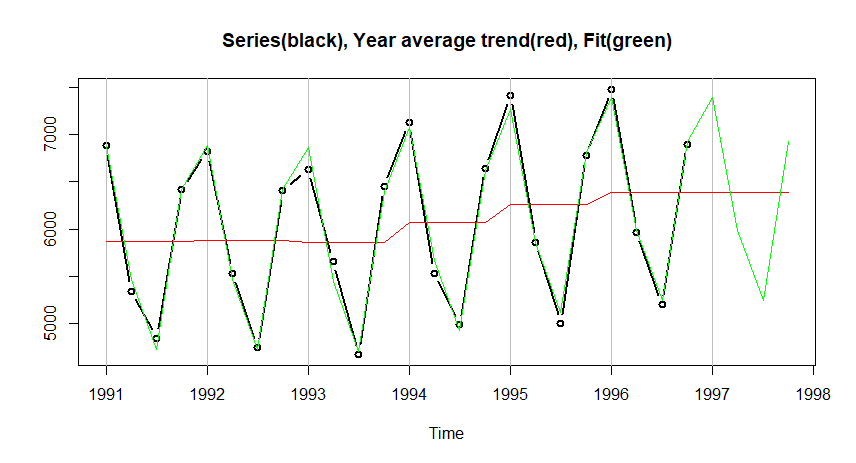
\includegraphics[width=\textwidth]{3.png}
\end{figure}

下图为去掉了趋势后的序列、季节项、取掉了趋势与季节项后的随机项:
\begin{lstlisting}[language=r]
> plot.season(y.detrended, seas0)
\end{lstlisting}
\begin{figure}[H]
	\centering
	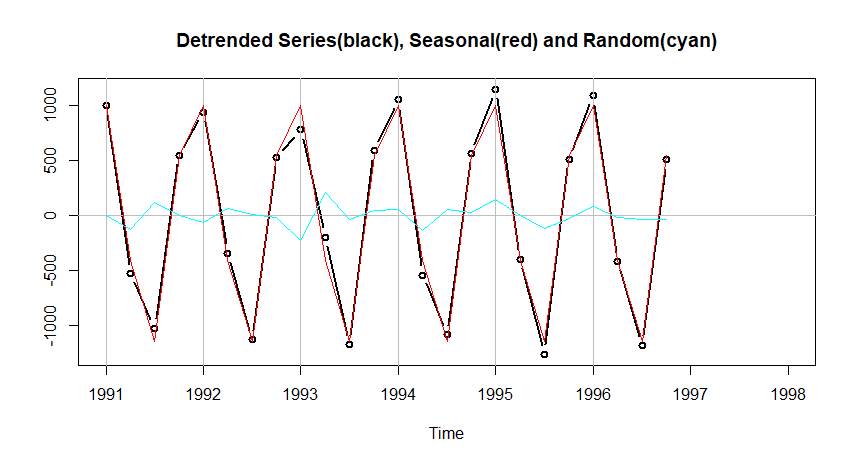
\includegraphics[width=\textwidth]{4.png}
\end{figure}

\subsubsection{用时间的线性回归作为趋势项估计, 季度平均作为季节项}
可以设趋势为$ T_t = a + bt $,用一元线性回归程序估计趋势并预测。下图绘制了
原始数据、估计的趋势、拟合值(包括趋势与季节项):
\begin{lstlisting}[language=r]
> yy <- c(y)
> tt <- seq(length(y))
> lmr <- lm(yy ~ tt)
> tr.more <- ts(predict(lmr, newdata=list(tt=seq(length(y)+4))),
+               frequency=4, start=c(1991,1))
> ## season
> y.detrended <- y - tr.more[1:length(y)]
> seas0 <- get.season(y.detrended)
> seas.more <- ts(rep(seas0, 7),
+                 start=start(y), frequency=4)
> y.pred <- tr.more + seas.more
> plot(ymore, main="Series(black), Linear trend(red) and Fit(green)",
+      lwd=2,
+      type="b", col="black")
> lines(tr.more, col="red", type="l")
> lines(y.pred, col="green", type="l")
\end{lstlisting}
\begin{figure}[H]
	\centering
	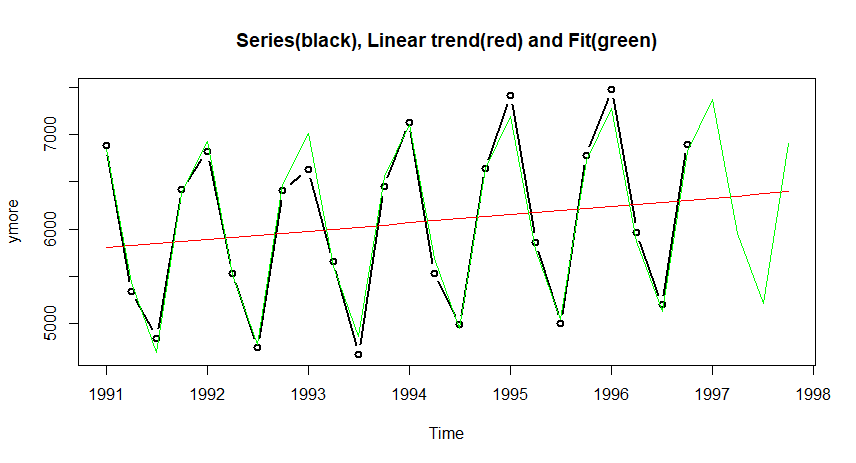
\includegraphics[width=\textwidth]{5.png}
\end{figure}

\textbf{lm()}是R语言中经常用到的函数,用来拟合回归模型。它是拟合线性模型最基本的函数。\\

下图为去掉了趋势后的序列、季节项、取掉了趋势与季节项后的随机项:
\begin{lstlisting}[language=r]
> plot.season(y.detrended, seas0)
\end{lstlisting}
\begin{figure}[H]
	\centering
	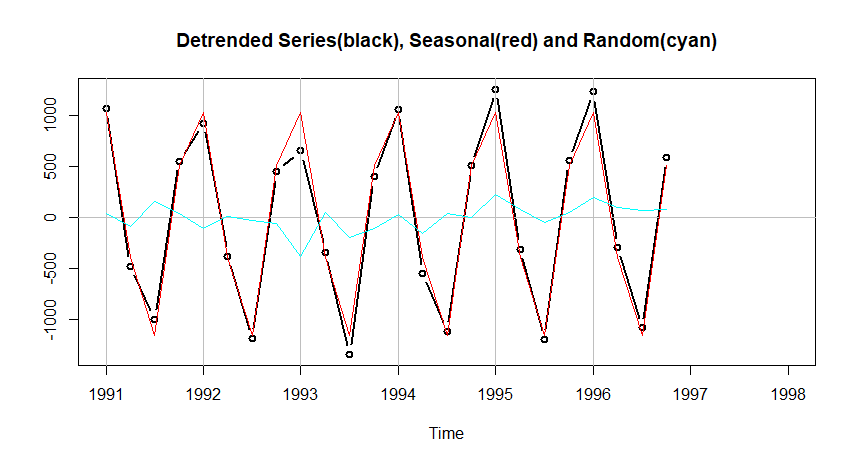
\includegraphics[width=\textwidth]{6.png}
\end{figure}

\subsubsection{二次曲线趋势}
可以用$ T_t = a+bt+ct^2 $ 作为趋势模型,用多元线性回归程序估计模型并预测。
下图绘制了原始数据、估计的趋势、拟合值(包括趋势与季节项):
\begin{lstlisting}[language=r]
> yy <- c(y)
> tt <- seq(length(y))
> lmr <- lm(yy ~ tt + I(tt^2))
> tr.more <- ts(predict(lmr, new.data=list(tt=seq(length(y)+4))),
+               frequency=4, start=c(1991,1))
> ## season
> y.detrended <- y - tr.more[1:length(y)]
> seas0 <- get.season(y.detrended)
> seas.more <- ts(rep(seas0, 7),
+                 start=start(y), frequency=4)
> y.pred <- tr.more + seas.more
> plot(ymore, main="Series(black), Quadratic trend(red) and Fit(cyan)",
+      lwd=2,
+      type="b", col="black")
> lines(tr.more, col="red", type="l")
> lines(y.pred, col="green", type="l")
\end{lstlisting}
\begin{figure}[H]
	\centering
	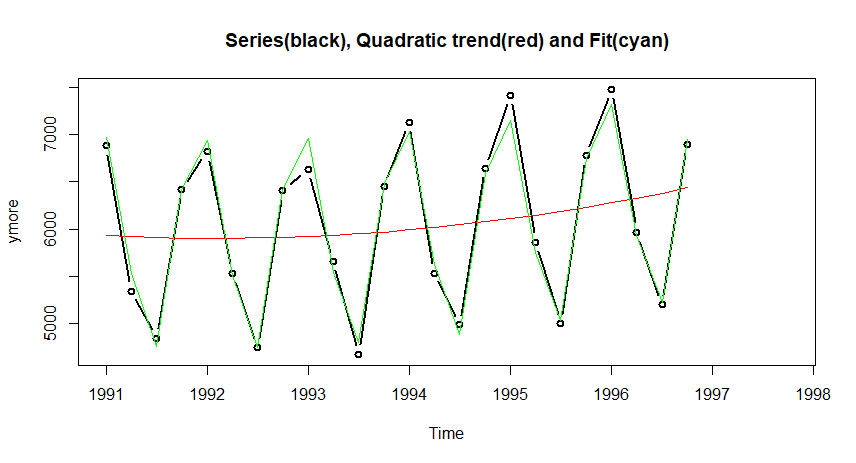
\includegraphics[width=\textwidth]{7.png}
\end{figure}
下图为去掉了趋势后的序列、季节项、取掉了趋势与季节项后的随机项:
\begin{lstlisting}[language=r]
> plot.season(y.detrended, seas0)
\end{lstlisting}
\begin{figure}[H]
	\centering
	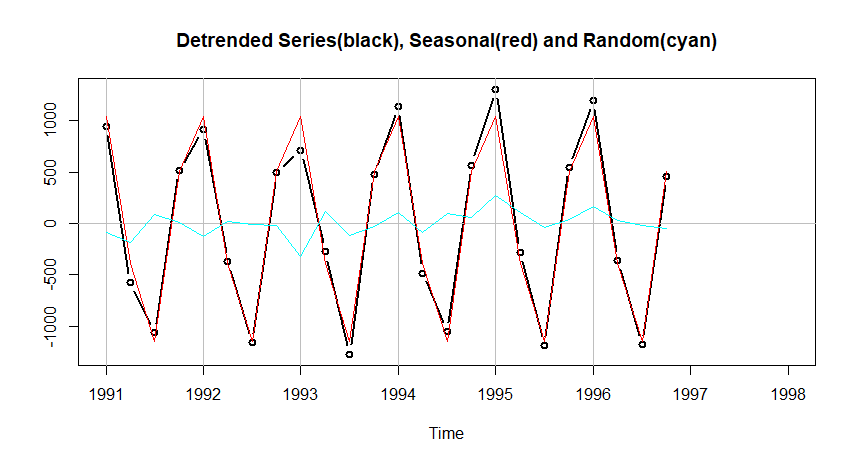
\includegraphics[width=\textwidth]{8.png}
\end{figure}

\subsubsection{decompose() 函数}
R 的stats 包的\textbf{decompose()} 函数输入一个时间序列,将其分解为趋势项、季
节项和随机项。去趋势的方法是中心对称滑动平均。可以用type="additive"
或type="multiplicative" 指定各项之间是相加还是相乘。

下图分别是原始序列、趋势估计、季节项估计和随机项估计。函数输出结果为一个
列表,各项为x, seasonal, trend, random 等。
\begin{lstlisting}[language=r]
> res1 <- decompose(coal.consumption)
> plot(res1)
\end{lstlisting}
\begin{figure}[H]
	\centering
	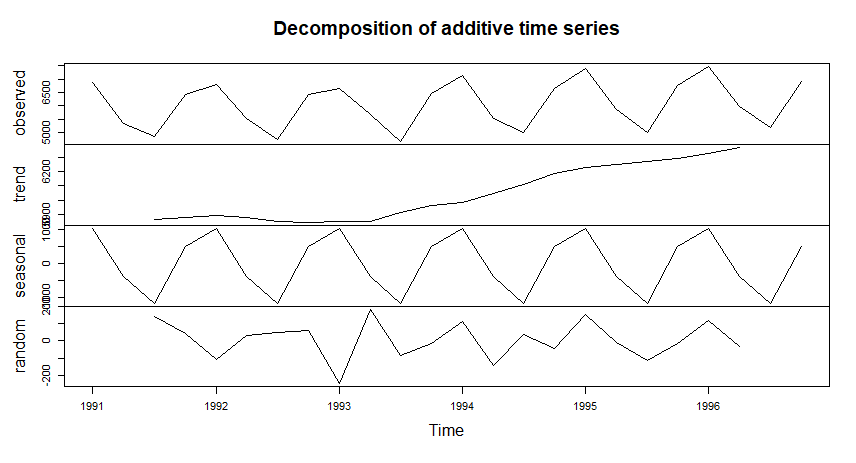
\includegraphics[width=\textwidth]{9.png}
\end{figure}

又比如,考虑著名的美国泛美航空公司1949-1960 的国际航班订票数的月度数
据(单位:千人),12 年144 个月的数据。序列图:
\begin{lstlisting}[language=r]
> plot(AirPassengers)
\end{lstlisting}
\begin{figure}[H]
	\centering
	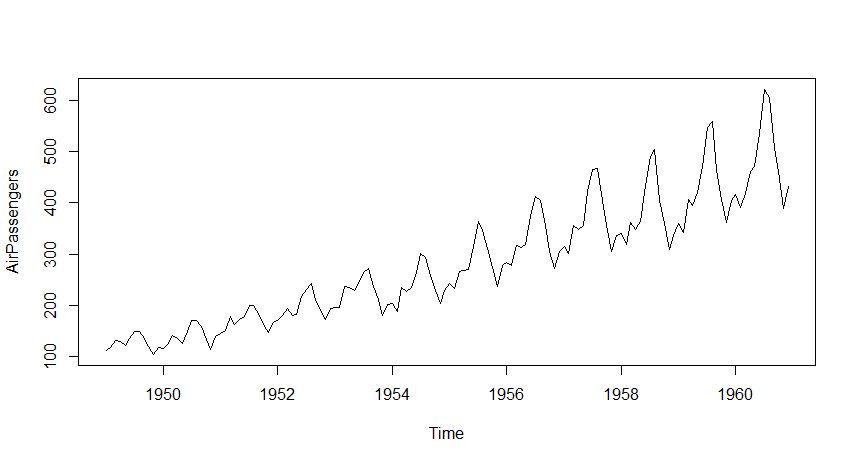
\includegraphics[width=\textwidth]{10.png}
\end{figure}
分解:
\begin{lstlisting}[language=r]
> plot(decompose(AirPassengers, type="multiplicative"))
\end{lstlisting}
\begin{figure}[H]
	\centering
	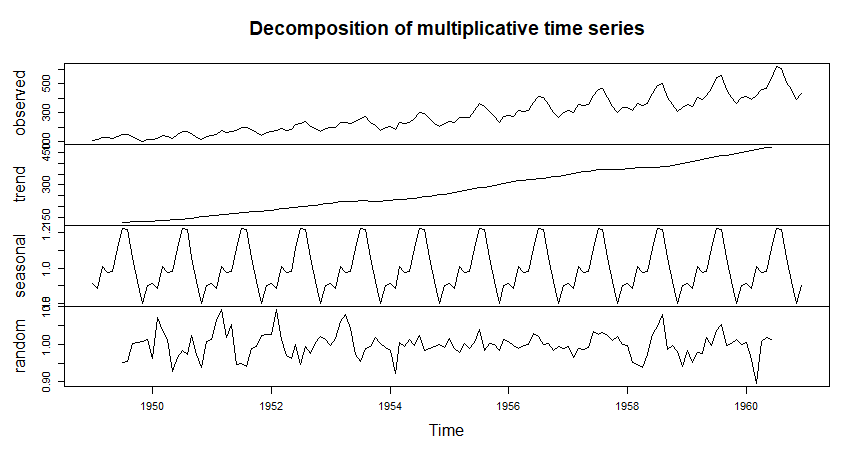
\includegraphics[width=\textwidth]{11.png}
\end{figure}
\section{平稳序列}
\subsection{白噪声}
\subsubsection{模拟的Poisson 白噪声}

\begin{lstlisting}[language=r]
> set.seed(1); x <- rpois(100, 1)
> plot(x, type="h", xlab="time", ylab="", main="Poisson White Noise")
\end{lstlisting}
\begin{figure}[H]
	\centering
	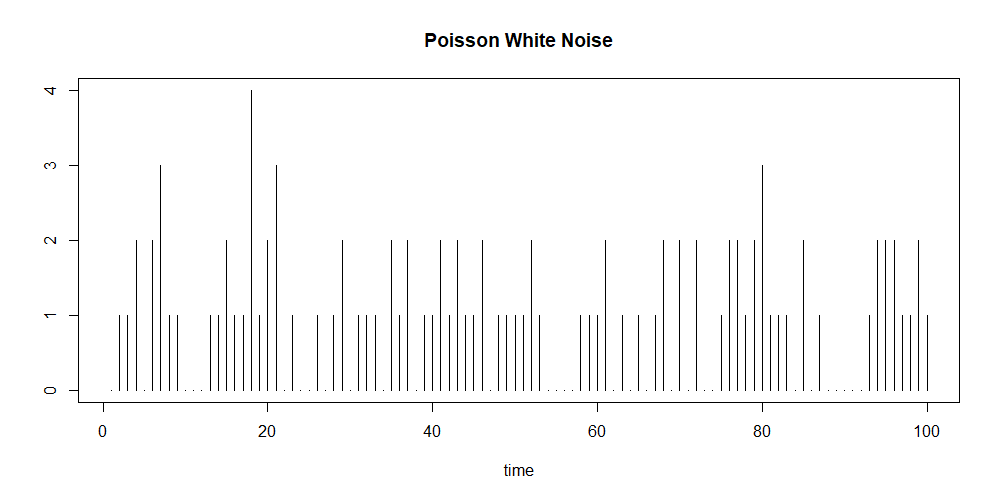
\includegraphics[width=\textwidth]{12.png}
\end{figure}
\subsubsection{模拟的标准正态白噪声}
\begin{lstlisting}[language=r]
> set.seed(1); x <- rnorm(100)
> plot(x, type="h", xlab="time", ylab="", main="Gaussian White Noise")
\end{lstlisting}
\begin{figure}[H]
	\centering
	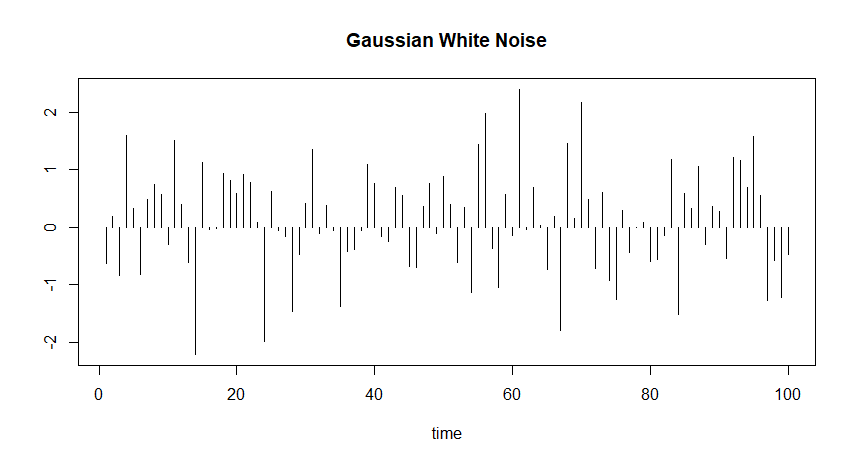
\includegraphics[width=\textwidth]{13.png}
\end{figure}
\subsubsection{模拟的随机相位白噪声}
\begin{lstlisting}[language=r]
> x <- cos(2*pi/12*(1:100) + runif(100, 0, 2*pi))
> plot(x, type="l", xlab="time", ylab="",
+      main="Random Phase White Noise")
\end{lstlisting}
\begin{figure}[H]
	\centering
	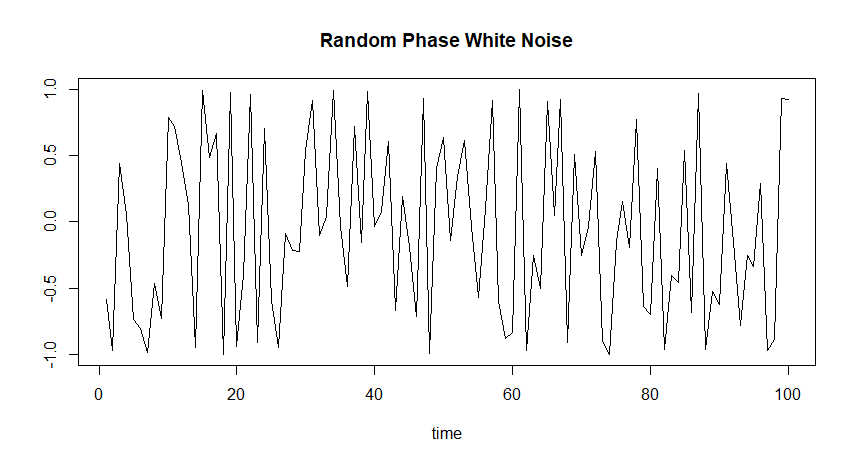
\includegraphics[width=\textwidth]{14.png}
\end{figure}

\chapter{线性平稳序列和线性滤波}
\section{有限运动平均}
\subsection{例:余弦波信号的滤波}
\begin{lstlisting}[language=r]
> demo.mafilt <- function(b=3, M=3){
	+     n <- 100
	+     ##om <- pi/7
	+     om <- pi/12
	+     sigma <- 1.0
	+     eps <- rnorm(n, 0, sigma)
	+     sn0 <- b^2 / (2*sigma^2)
	+     tt <- seq(n)
	+     u <- runif(1)
	+     signal <- b * cos(om*tt + 2*pi*u)
	+     y <- signal + eps
	+     filt <- rep(1/(2*M+1), 2*M+1)
	+     yf <- filter(y, filt, method="convolution")
	+     rg <- range(c(y, yf))
	+     sn <- round(b^2 / (2*sigma^2), 3)
	+     plot(tt, y, main=paste("MA filter: SN=", sn, sep=""),
	+          type="l", xlab='time', ylab='y',
	+          xlim=c(0,120),
	+          ylim=c(-b*1.5,b*1.5))
	+     lines(tt, signal, col="green", lwd=2)
	+     lines(tt, yf, col="red", lwd=2)
	+     legend("topright", lty=c(1,1,1), lwd=c(1,2,2),
	+            col=c("black", "green", "red"),
	+            legend=c(" 序列", " 信号", " 滤波"))
	+ }
> demo.mafilt()
\end{lstlisting}
\begin{figure}[H]
	\centering
	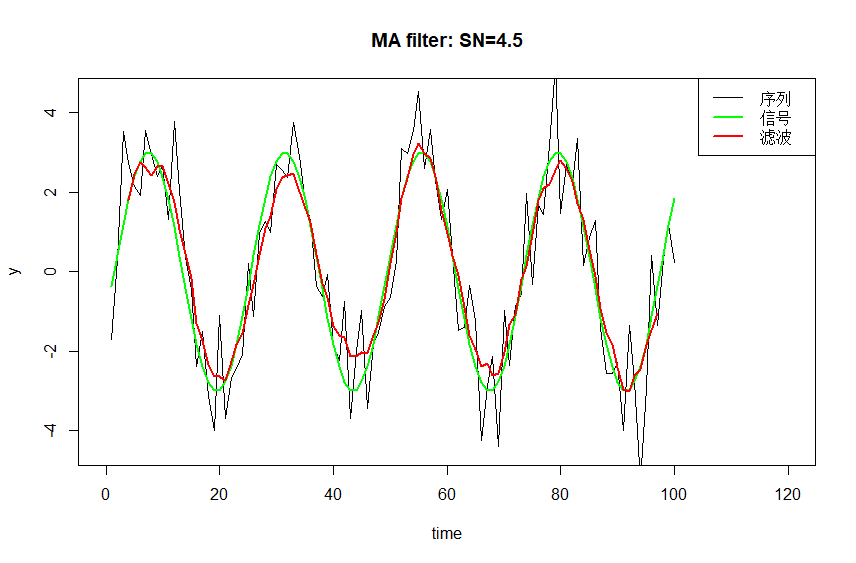
\includegraphics[width=\textwidth]{15.png}
\end{figure}

\chapter{自回归模型及其平稳性}
\section{AR(1)}

\begin{lstlisting}[language=r]
> ar1.gen <- function(n, a, sigma=1.0,
+                     plot.it=FALSE, n0=1000,
+                     x0=numeric(length(a))){
	+     n2 <- n0 + n
	+     eps <- rnorm(n2, 0, sigma)
	+     x2 <- filter(eps, a, method="recursive", side=1, init=x0)
	+     x <- x2[(n0+1):n2]
	+     x <- ts(x)
	+ attr(x, "model") <- "AR(1)"
	+ attr(x, "a") <- a
	+ attr(x, "sigma") <- sigma
	+ if(plot.it) plot(x)
	+ x
	+ }
> demo.ar1 <- function(){
	+     as <- c(0.1, 0.3, 0.5, 0.6, 0.7, 0.8, 0.9, 0.95, 0.99, 1.0, 1.001)
	+     x0 <- 10
	+     n <- 500
	+     for(a in as){
	  +         for(a1 in c(a, -a)){
		+         x <- ar1.gen(n=n, a=a1, sigma=0.2,
		+                      n0=0, x0=x0)
		+         plot(x, main=paste("AR(1): x0=10, a=", a1, sep=""),		
		+              ylim=c(-12, 15))
		+         abline(h=0, col="red")
		+       }
	+     }
 + }
> set.seed(106)
> demo.ar1()
\end{lstlisting}

\begin{tcolorbox}[colback=pink!10!white,colframe=pink!100!black]
	\textbf{filter(x, filter, method = c("convolution", "recursive"), sides = 2, circular = FALSE, init)}
	\begin{itemize}
		\item x: 一元或多元时间序列。
		\item filter: 一个反向的时间顺序滤波器系数向量(AR或MA系数)。
		\item method: "convolution"或者"recursive"(可以缩写),如果是"convolution"则是移动平均,如果是"recursive"则是自回归。
		\item sides: 卷积过滤器。如果sides=1滤波器系数是对过去的价值观;如果sides=2他们周围滞后0为中心的。在这种情况下,过滤器的长度应为奇数,但如果它是偶数,过滤器的更多的是向前的时间比落后。
		\item circular: 卷积过滤器。如果TRUE,包装左右两端系列的过滤,否则假定缺少外部值(NA)。
		\item init: 只有递归滤波器。指定的时间序列的初始值,只是之前的起始值,反向时间顺序。默认的是一套零。
	\end{itemize}
\end{tcolorbox}
\begin{tcolorbox}[colback=pink!10!white,colframe=pink!100!black]
用\textbf{attr(x, "属性名")}的格式读取或定义x的属性。可以让向量x额外地保存一个theta属性, 这样的属性常常成为“元数据”(meta data), 比如, 用来保存数据的说明、模拟数据的真实模型参数,等等。

\end{tcolorbox}
\begin{figure}[H]
	\centering
	\subfigure{
		\begin{minipage}[t]{0.5\textwidth}
			\centering
			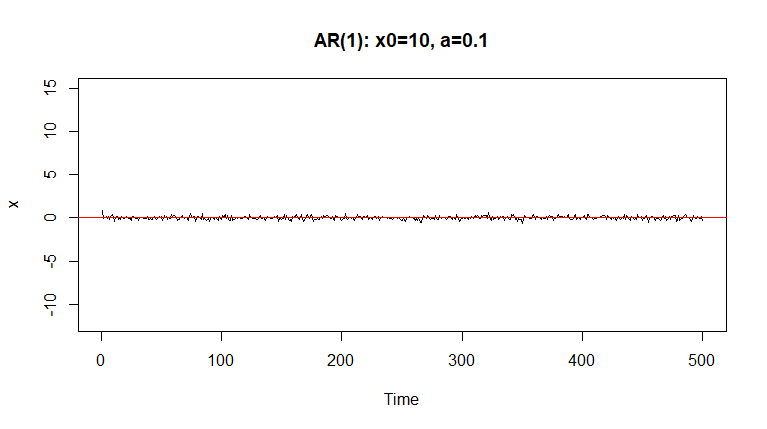
\includegraphics[width=8cm]{16.png}
		\end{minipage}%
	}%
	\subfigure{
		\begin{minipage}[t]{0.5\textwidth}
			\centering
			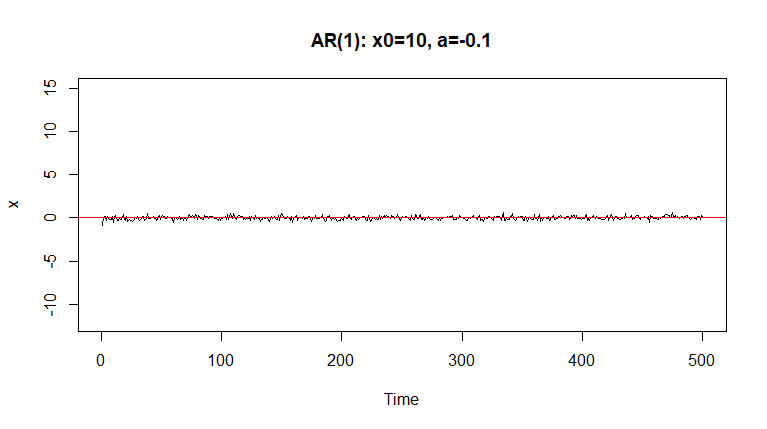
\includegraphics[width=8cm]{17.png}
	\end{minipage}}
\end{figure}
\begin{figure}[H]
	\centering
	\subfigure{
		\begin{minipage}[t]{0.5\textwidth}
			\centering
			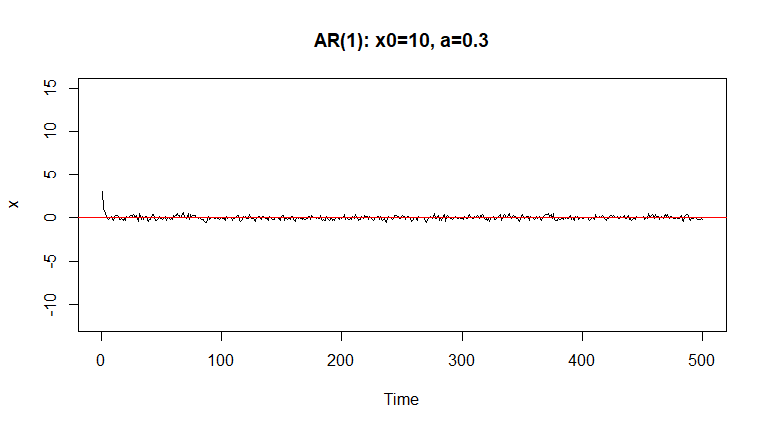
\includegraphics[width=8cm]{18.png}
		\end{minipage}%
	}%
	\subfigure{
		\begin{minipage}[t]{0.5\textwidth}
			\centering
			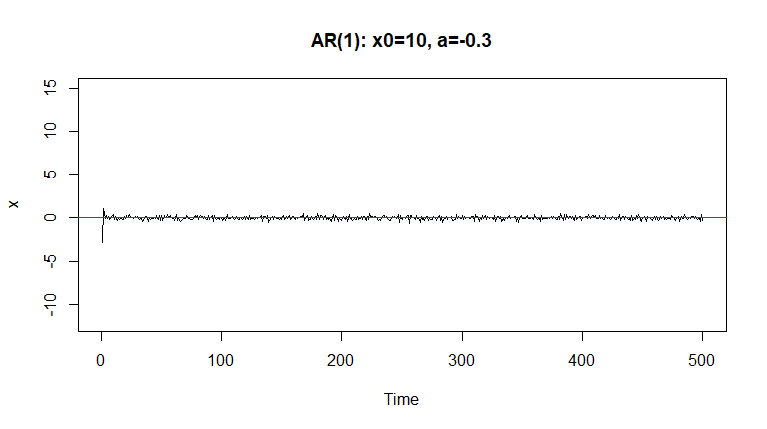
\includegraphics[width=8cm]{19.png}
	\end{minipage}}
\end{figure}
\begin{figure}[H]
	\centering
	\subfigure{
		\begin{minipage}[t]{0.5\textwidth}
			\centering
			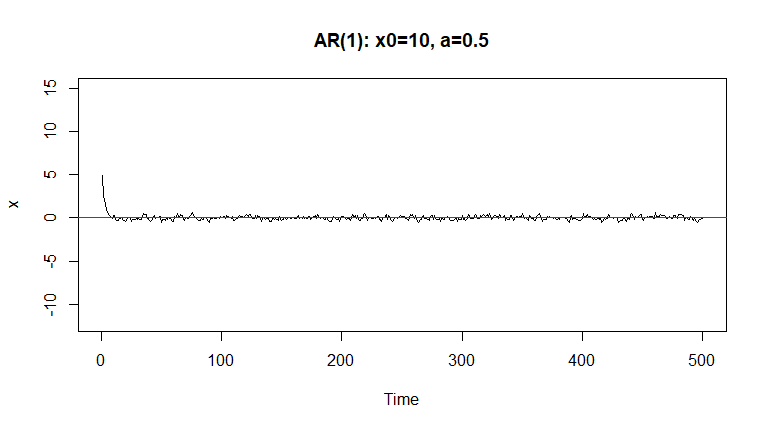
\includegraphics[width=8cm]{20.png}
		\end{minipage}%
	}%
	\subfigure{
		\begin{minipage}[t]{0.5\textwidth}
			\centering
			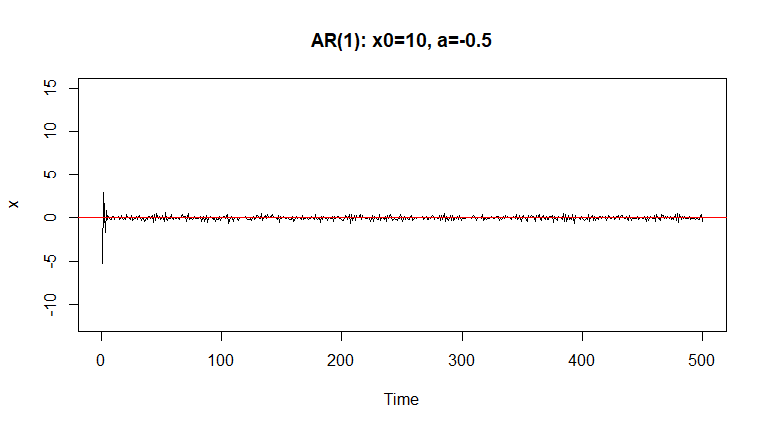
\includegraphics[width=8cm]{21.png}
	\end{minipage}}
\end{figure}
\begin{figure}[H]
	\centering
	\subfigure{
		\begin{minipage}[t]{0.5\textwidth}
			\centering
			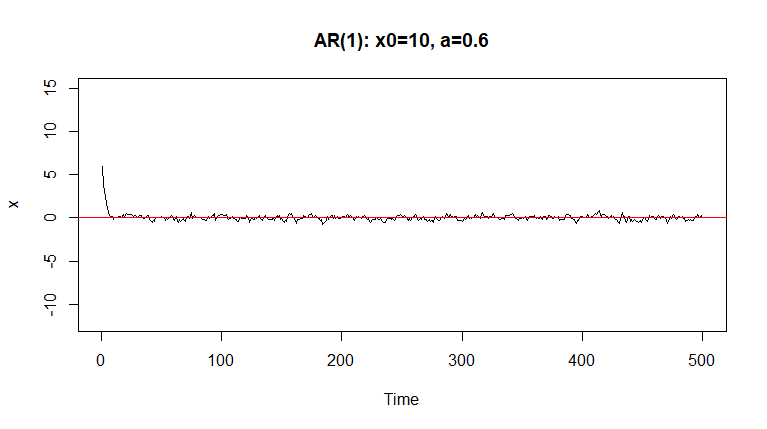
\includegraphics[width=8cm]{22.png}
		\end{minipage}%
	}%
	\subfigure{
		\begin{minipage}[t]{0.5\textwidth}
			\centering
			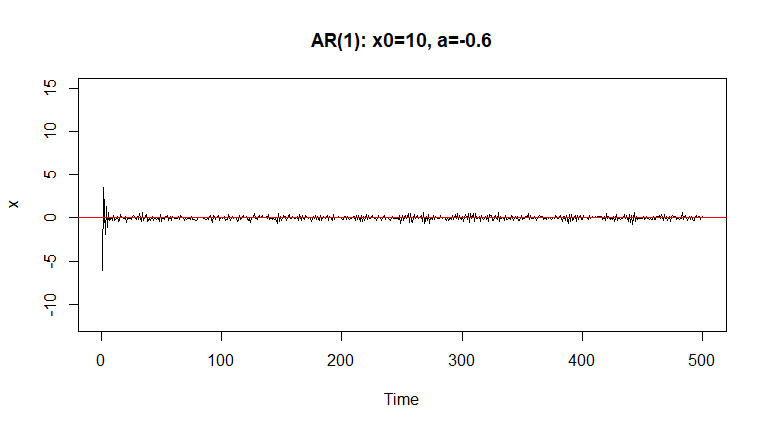
\includegraphics[width=8cm]{23.png}
	\end{minipage}}
\end{figure}
\begin{figure}[H]
	\centering
	\subfigure{
		\begin{minipage}[t]{0.5\textwidth}
			\centering
			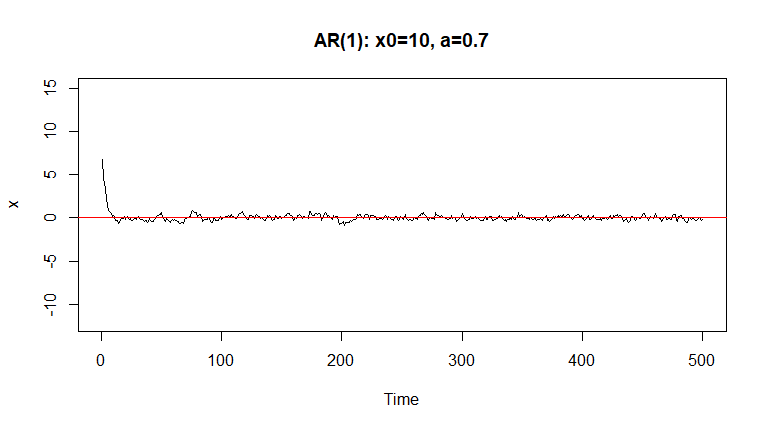
\includegraphics[width=8cm]{24.png}
		\end{minipage}%
	}%
	\subfigure{
		\begin{minipage}[t]{0.5\textwidth}
			\centering
			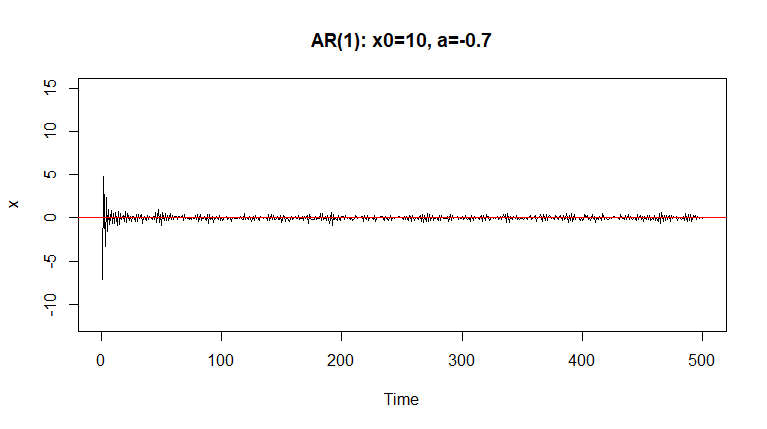
\includegraphics[width=8cm]{25.png}
	\end{minipage}}
\end{figure}
\begin{figure}[H]
	\centering
	\subfigure{
		\begin{minipage}[t]{0.5\textwidth}
			\centering
			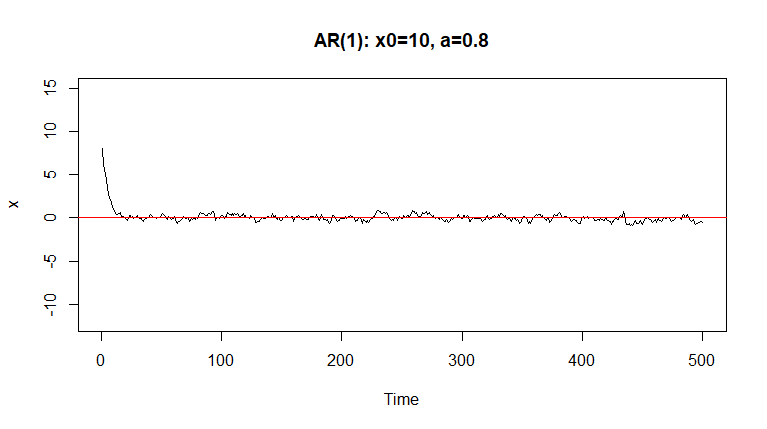
\includegraphics[width=8cm]{26.png}
		\end{minipage}%
	}%
	\subfigure{
		\begin{minipage}[t]{0.5\textwidth}
			\centering
			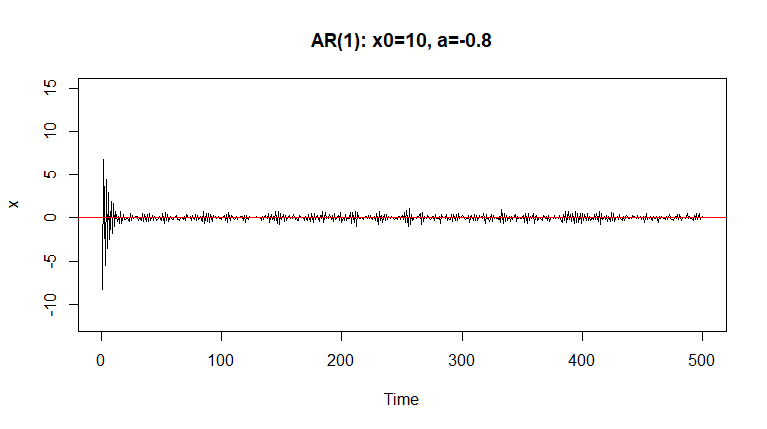
\includegraphics[width=8cm]{27.png}
	\end{minipage}}
\end{figure}
\begin{figure}[H]
	\centering
	\subfigure{
		\begin{minipage}[t]{0.5\textwidth}
			\centering
			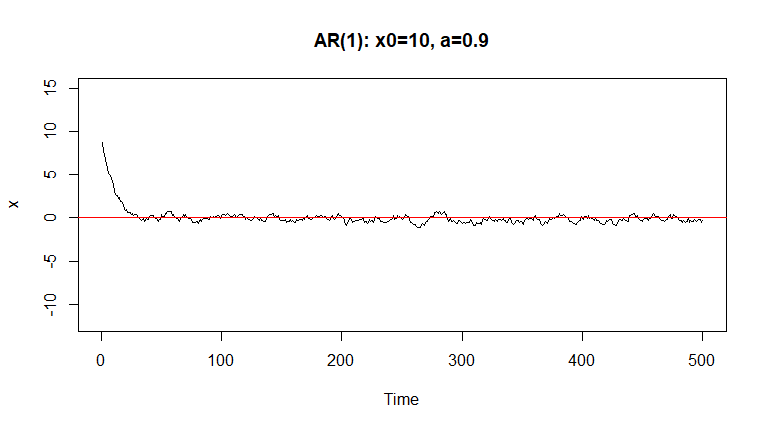
\includegraphics[width=8cm]{28.png}
		\end{minipage}%
	}%
	\subfigure{
		\begin{minipage}[t]{0.5\textwidth}
			\centering
			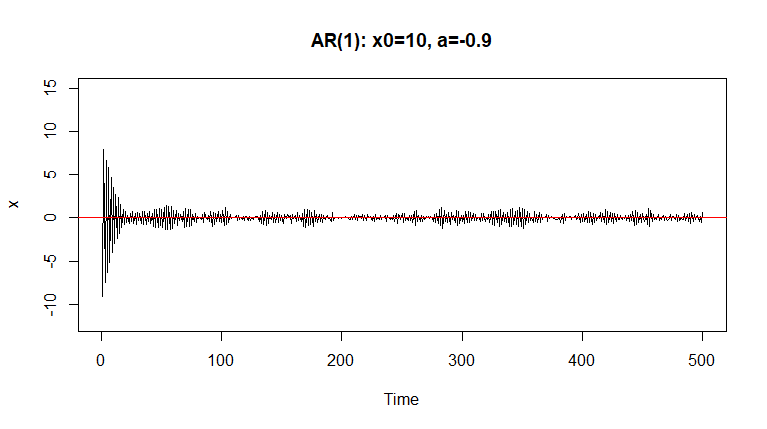
\includegraphics[width=8cm]{30.png}
	\end{minipage}}
\end{figure}
\begin{figure}[H]
	\centering
	\subfigure{
		\begin{minipage}[t]{0.5\textwidth}
			\centering
			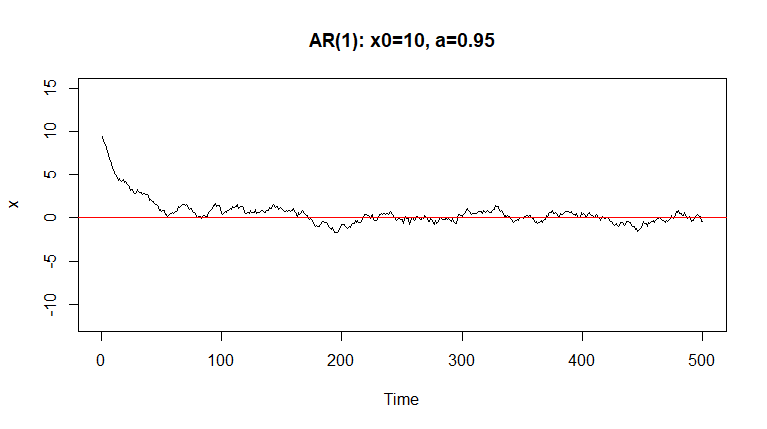
\includegraphics[width=8cm]{31.png}
		\end{minipage}%
	}%
	\subfigure{
		\begin{minipage}[t]{0.5\textwidth}
			\centering
			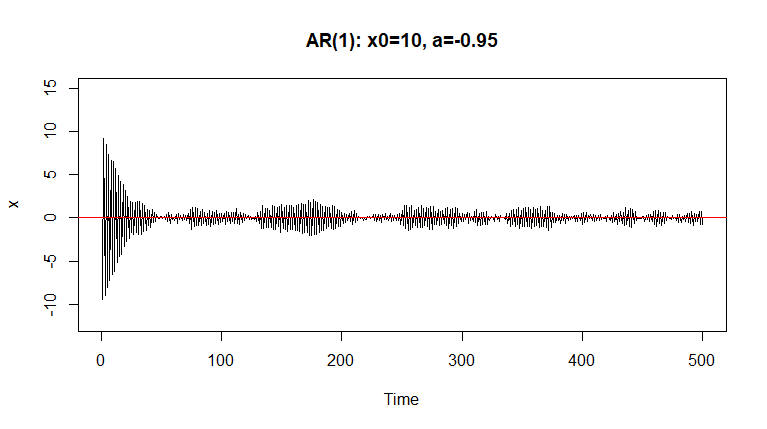
\includegraphics[width=8cm]{32.png}
	\end{minipage}}
\end{figure}
\begin{figure}[H]
	\centering
	\subfigure{
		\begin{minipage}[t]{0.5\textwidth}
			\centering
			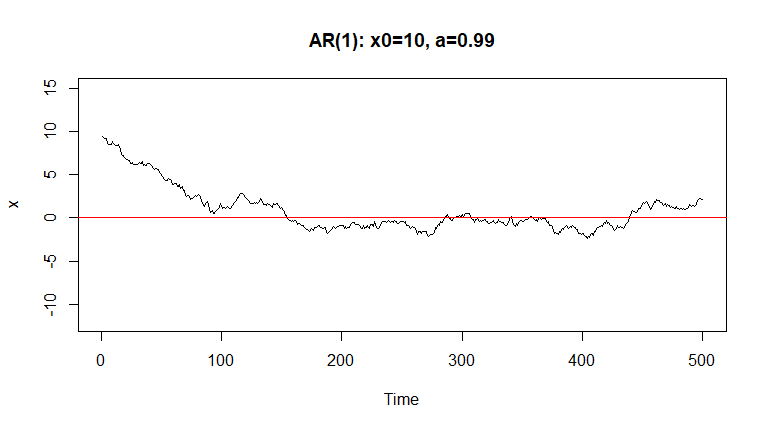
\includegraphics[width=8cm]{33.png}
		\end{minipage}%
	}%
	\subfigure{
		\begin{minipage}[t]{0.5\textwidth}
			\centering
			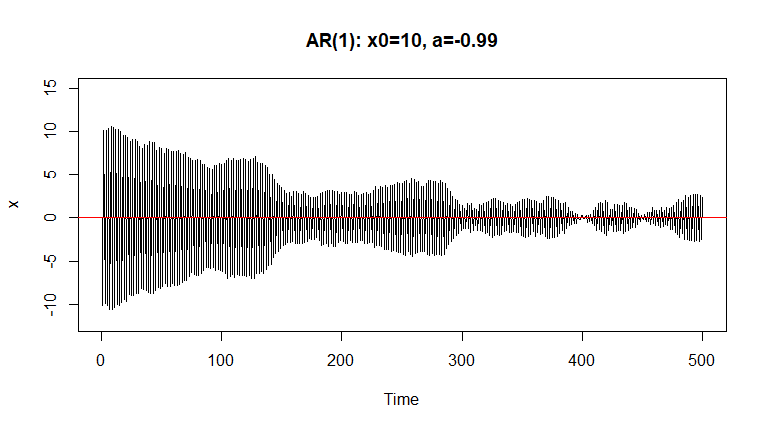
\includegraphics[width=8cm]{34.png}
	\end{minipage}}
\end{figure}
\begin{figure}[H]
	\centering
	\subfigure{
		\begin{minipage}[t]{0.5\textwidth}
			\centering
			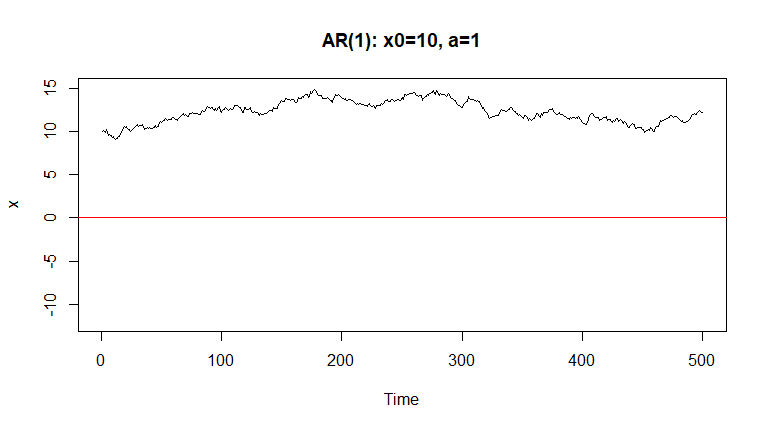
\includegraphics[width=8cm]{35.png}
		\end{minipage}%
	}%
	\subfigure{
		\begin{minipage}[t]{0.5\textwidth}
			\centering
			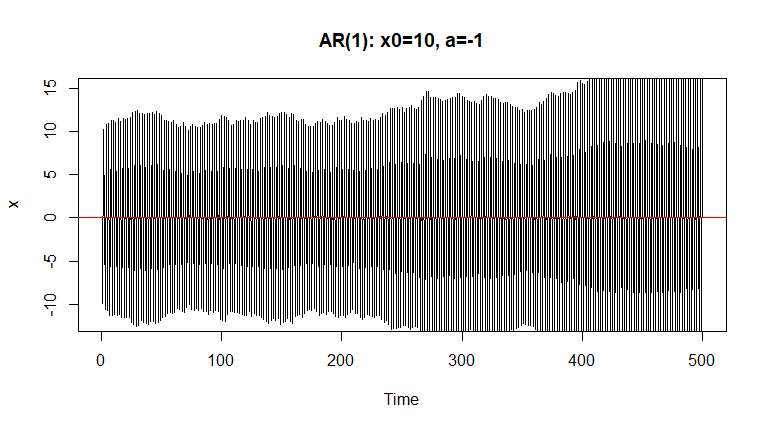
\includegraphics[width=8cm]{36.png}
	\end{minipage}}
\end{figure}
\begin{figure}[H]
	\centering
	\subfigure{
		\begin{minipage}[t]{0.5\textwidth}
			\centering
			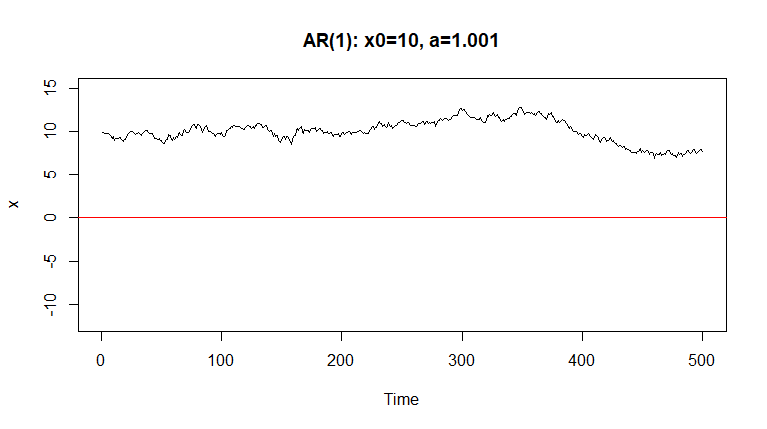
\includegraphics[width=8cm]{37.png}
		\end{minipage}%
	}%
	\subfigure{
		\begin{minipage}[t]{0.5\textwidth}
			\centering
			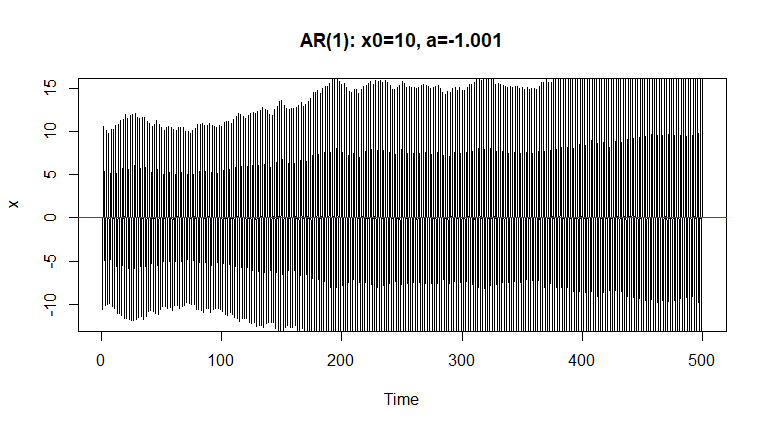
\includegraphics[width=8cm]{38.png}
	\end{minipage}}
\end{figure}



\begin{lstlisting}[language=r]
	
\end{lstlisting}
\begin{lstlisting}[language=r]
	
\end{lstlisting}
\begin{lstlisting}[language=r]
	
\end{lstlisting}
\begin{lstlisting}[language=r]
	
\end{lstlisting}
\begin{lstlisting}[language=r]
	
\end{lstlisting}
\begin{lstlisting}[language=r]
	
\end{lstlisting}
\begin{lstlisting}[language=r]
	
\end{lstlisting}
\begin{lstlisting}[language=r]
	
\end{lstlisting}
\begin{lstlisting}[language=r]
	
\end{lstlisting}
\begin{lstlisting}[language=r]
	
\end{lstlisting}
\begin{lstlisting}[language=r]
	
\end{lstlisting}
\begin{lstlisting}[language=r]
	
\end{lstlisting}
\begin{lstlisting}[language=r]
	
\end{lstlisting}
\begin{lstlisting}[language=r]
	
\end{lstlisting}
\begin{lstlisting}[language=r]
	
\end{lstlisting}
\begin{lstlisting}[language=r]
	
\end{lstlisting}
\begin{lstlisting}[language=r]
	
\end{lstlisting}
\begin{lstlisting}[language=r]
	
\end{lstlisting}
\begin{lstlisting}[language=r]
	
\end{lstlisting}
\begin{lstlisting}[language=r]
	
\end{lstlisting}
\begin{lstlisting}[language=r]
	
\end{lstlisting}
\begin{lstlisting}[language=r]
	
\end{lstlisting}
\begin{lstlisting}[language=r]
	
\end{lstlisting}
\begin{lstlisting}[language=r]
	
\end{lstlisting}
\begin{lstlisting}[language=r]
	
\end{lstlisting}
\begin{lstlisting}[language=r]
	
\end{lstlisting}
\begin{lstlisting}[language=r]
	
\end{lstlisting}
\begin{lstlisting}[language=r]
	
\end{lstlisting}
\begin{lstlisting}[language=r]
	
\end{lstlisting}
\begin{lstlisting}[language=r]
	
\end{lstlisting}
\begin{lstlisting}[language=r]
	
\end{lstlisting}
\begin{lstlisting}[language=r]
	
\end{lstlisting}
\begin{lstlisting}[language=r]
	
\end{lstlisting}
\begin{lstlisting}[language=r]
	
\end{lstlisting}
\begin{lstlisting}[language=r]
	
\end{lstlisting}
\begin{lstlisting}[language=r]
	
\end{lstlisting}
\begin{lstlisting}[language=r]
	
\end{lstlisting}
\begin{lstlisting}[language=r]
	
\end{lstlisting}
\begin{lstlisting}[language=r]
	
\end{lstlisting}
\begin{lstlisting}[language=r]
	
\end{lstlisting}

\end{document}